\documentclass{beamer}
\usetheme{Dresden}

\usepackage{fontspec}
\usepackage{kpfonts}
\usepackage{graphicx}
\usepackage{pgfplots}
\usepackage{pgfplotstable}
\usepackage{tikz}
\usetikzlibrary{arrows,automata,mindmap,shapes,positioning,patterns,snakes,calc}

\pgfplotsset{every x tick label/.append style={font=\small, yshift=0.2ex}}
\pgfplotsset{every y tick label/.append style={font=\small, xshift=0.2ex}}


\usepackage{amsmath,amsthm,bm}
\usepackage{array}
\usepackage{color}
\usepackage{hyperref}

%\usepackage{algorithm}
%\usepackage{algpseudocode}
\usepackage{algorithm2e}


\hypersetup{
    colorlinks=true,
    linkcolor=blue,
    filecolor=blue,      
    urlcolor=blue,
}

\setbeamertemplate{caption}{\raggedright\insertcaption\par}
\usefonttheme[onlymath]{serif}
\usepackage{ragged2e}
\addtobeamertemplate{block begin}{}{\justifying}

\DeclareMathOperator*{\argmax}{\mathrm{\arg\max}}
\DeclareMathOperator*{\argmin}{\mathrm{\arg\min}}
\DeclareMathOperator*{\arginf}{\mathrm{\arg\inf}}
\DeclareMathOperator*{\argsup}{\mathrm{\arg\sup}}
\DeclareMathOperator{\sgn}{\mathrm{sgn}}
\DeclareMathOperator{\ind}{\mathrm{I}}
\DeclareMathOperator{\complex}{\mathrm{O}}
\DeclareMathOperator{\diag}{\mathrm{diag}}
\DeclareMathOperator{\prob}{\mathrm{Pr}}
\DeclareMathOperator{\var}{\mathrm{var}}
\DeclareMathOperator{\corr}{\mathrm{corr}}
\DeclareMathOperator{\cov}{\mathrm{cov}}
\DeclareMathOperator{\rand}{\mathrm{rand}}
\DeclareMathOperator{\vect}{\textit{vec}}
\DeclareMathOperator{\rank}{\textit{rank}}
\DeclareMathOperator{\tr}{\textit{tr}}


\title[]{Collective Credit Allocation in Science}
\author[Hua-Wei Shen and Albert-L\'aszl\'o Barab\'asi]{Hua-Wei Shen and Albert-L\'aszl\'o Barab\'asi\\Presenter: Chunheng Jiang}
\date{}


\begin{document}

\begin{frame}
\titlepage
\end{frame}

\begin{frame}{Problem: Credit Allocation}
\begin{block}{}
Interdisciplinary collaboration has been a trend, e.g. the Human Genome Project.
Papers are the primary form of intellectual products. However, there is no general guideline to place authors. Different fields may have extremely different traditions (corresponding author, contribution or alphabetical ordering), and the length of the list also varies widely from a solo to a giant orchestra with over 5,000 authors~\cite{collaborations2015combined}.
\vskip 1em
To make accurate estimation of their contribution to a joint work, a.k.a the Credit Allocation Problem, a simple but effective algorithm was proposed~\cite{shen2014collective}.
\end{block}
\end{frame}

\begin{frame}{Algorithm}
\begin{block}{}
\begin{itemize}
\item Target Paper: $p_0$
\item Authors: $\mathcal A=\{a_1,a_2,\ldots,a_m\}$
\item Papers Citing: $\mathcal D=\{d_1,d_2,\ldots,d_l\}$
\item Papers Co-cited: $\mathcal P=\{\textcolor{red}{p_0},p_1,p_2,\ldots,p_n\}$
\end{itemize}

The credit shares of a coauthor is determined by whether she continues working with other coauthors on the topic of $p_0$. Here, the set $\mathcal D$ plays as a committee from the same community, and the citations are their votes. A bipartite network can be constructed. 
\end{block}
\end{frame}

\begin{frame}{Algorithm}
\begin{block}{}
The credit share of $a_i$ in $p_0$ is computed with the formula: 
\[c_i = \sum_{j=1}^n A_{ij}s_j,\]
where $A_{ij}$ is the credit $a_i$ earns from the cocited paper $p_j$, and each coauthor gets the same amount of shares from $p_j$. The relevance level (or cocitation strength) $s_j$ of $p_j$ to $p_0$ is defined as the number of documents in $\mathcal D$ referring both $p_0$ and $p_j$.
\end{block}
\end{frame}

\begin{frame}{Algorithm}
\begin{figure}[ht]
\centering
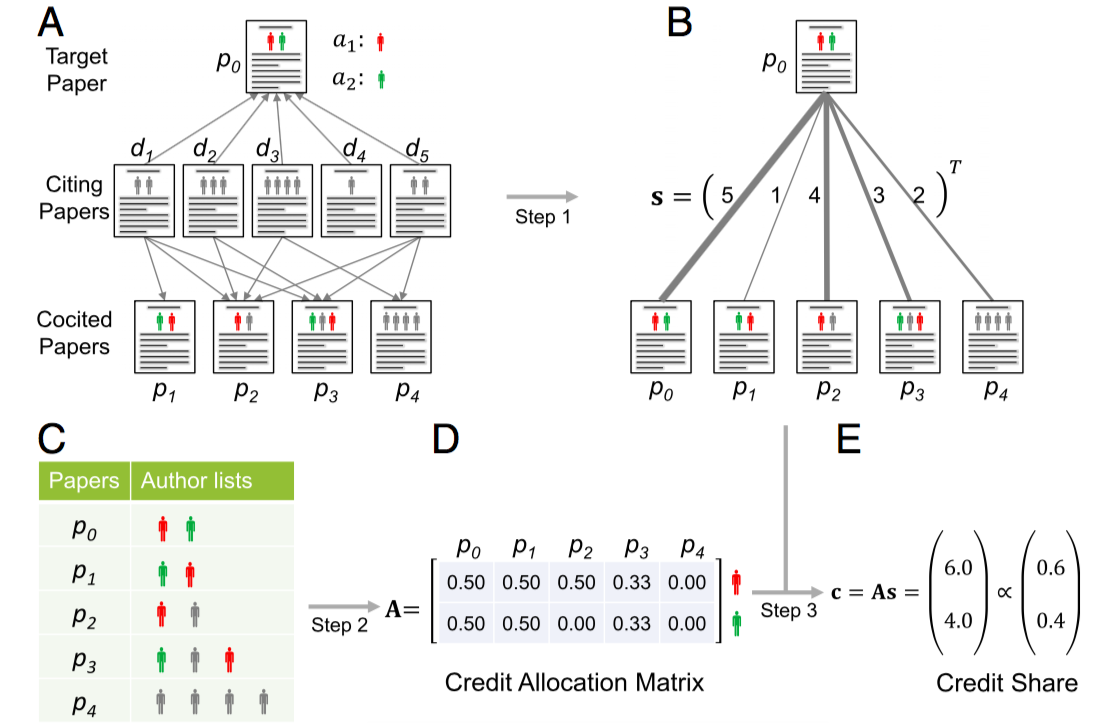
\includegraphics[scale=0.2]{figures/credalloc_algo}
\caption{Credit Allocation Algorithm}
\label{fig:algo}
\end{figure}
\end{frame}

\begin{frame}{Evaluation}
To evaluate the performance, the Nobel-prize winning papers in Physics (1995 - 2013), Chemistry (1998 - 2013), Medicine (2006 - 2013) and Economics (1998 - 2013) are collected to build the citation network. The credit allocation algorithm produces a credit share for each coauthor appeared in the awarding Nobel Prize papers.
\vskip 1em
The experimental results indicated that the algorithm performs very well, and successfully assigns the Nobel-prize winners the highest credit share in the awarding papers.
\end{frame}

\begin{frame}{Evaluation}

\begin{figure}[ht]
\centering
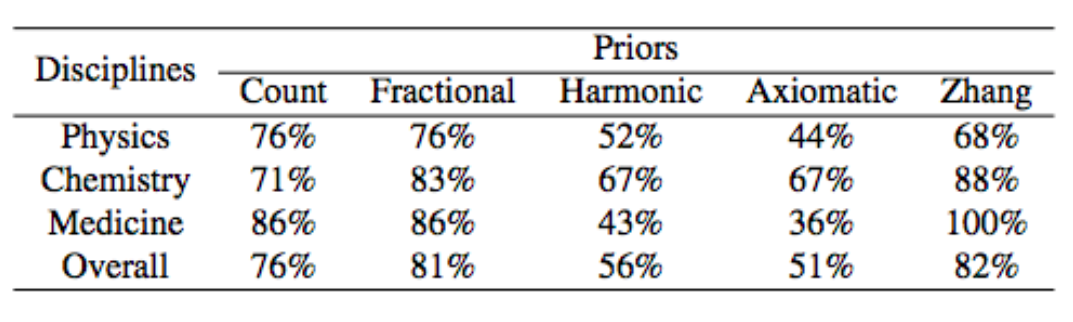
\includegraphics[scale=0.3]{figures/comparison}
\caption{Accuracy of the proposed algorithm with different prior rules for $A$}
\label{fig:nobel}
\end{figure}
\end{frame}


\begin{frame}{Evaluation}
\begin{figure}[ht]
\centering
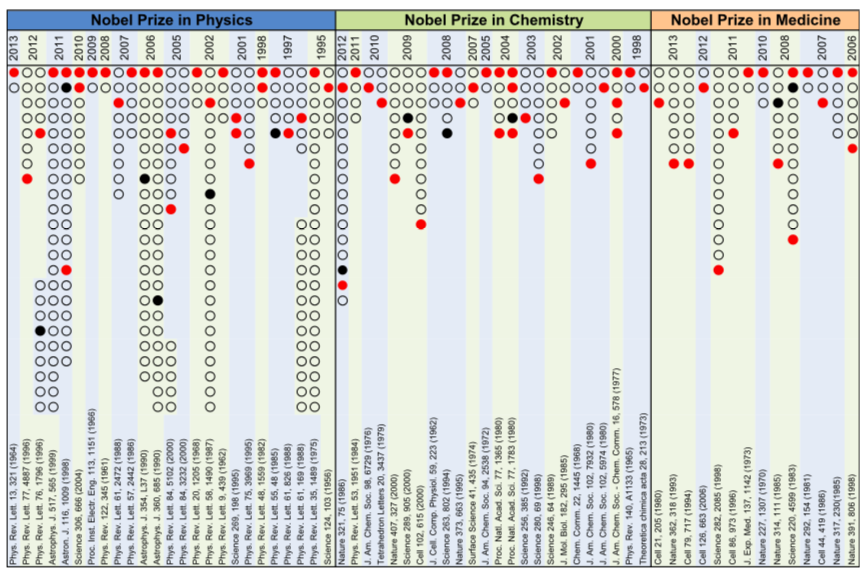
\includegraphics[scale=0.3]{figures/nobel}
\caption{Highest credit share earners (\tikz\draw[black,fill=black] (0,0) circle (.5ex);) and the Nobel Prize winners (\tikz\draw[red,fill=red] (0,0) circle (.5ex);)}
\label{fig:nobel}
\end{figure}
\end{frame}

\begin{frame}{Further Studies}
\begin{itemize}
\item Integrating both the order of coauthors and the contextual info to design better credit allocation matrix $A=(A_{ij})_{i=m}^{n+1}$
\item Differentiate the values of the citing papers $\mathcal D$ because of the reputation differences, produce more reliable relevance estimation of $s$ (link-analysis based analyze over all papers) 
%\item Evaluate the influence of scientists in multiple fields and identify the VIPs in the academia.
\item Authors' institutions and contextual text of the citation(definition, ideas)
\end{itemize}
\end{frame}

\begin{frame}[allowframebreaks]
\tiny\bibliography{references}
\bibliographystyle{unsrt}
\end{frame}

\end{document}